\chapter{Interfejs użytkownika, testy i podsumowanie}
\label{cha:gui-testy-podsumowanie}

\section{Projekt interfejsu użytkownika}

Interfejs użytkownika gry Godmist zaprojektowano zgodnie z zasadą minimalnej ingerencji w scenę gry. W widokach eksploracji oraz walki większość ekranu zajmuje właściwa scena, natomiast elementy HUD rozmieszczono przy krawędziach ekranu w formie lekkich widżetów. Bardziej rozbudowane okna, takie jak ekwipunek, dziennik zadań czy interakcje z NPC, otwierane są jako osobne nakładki.

\begin{figure}[H]
    \centering
    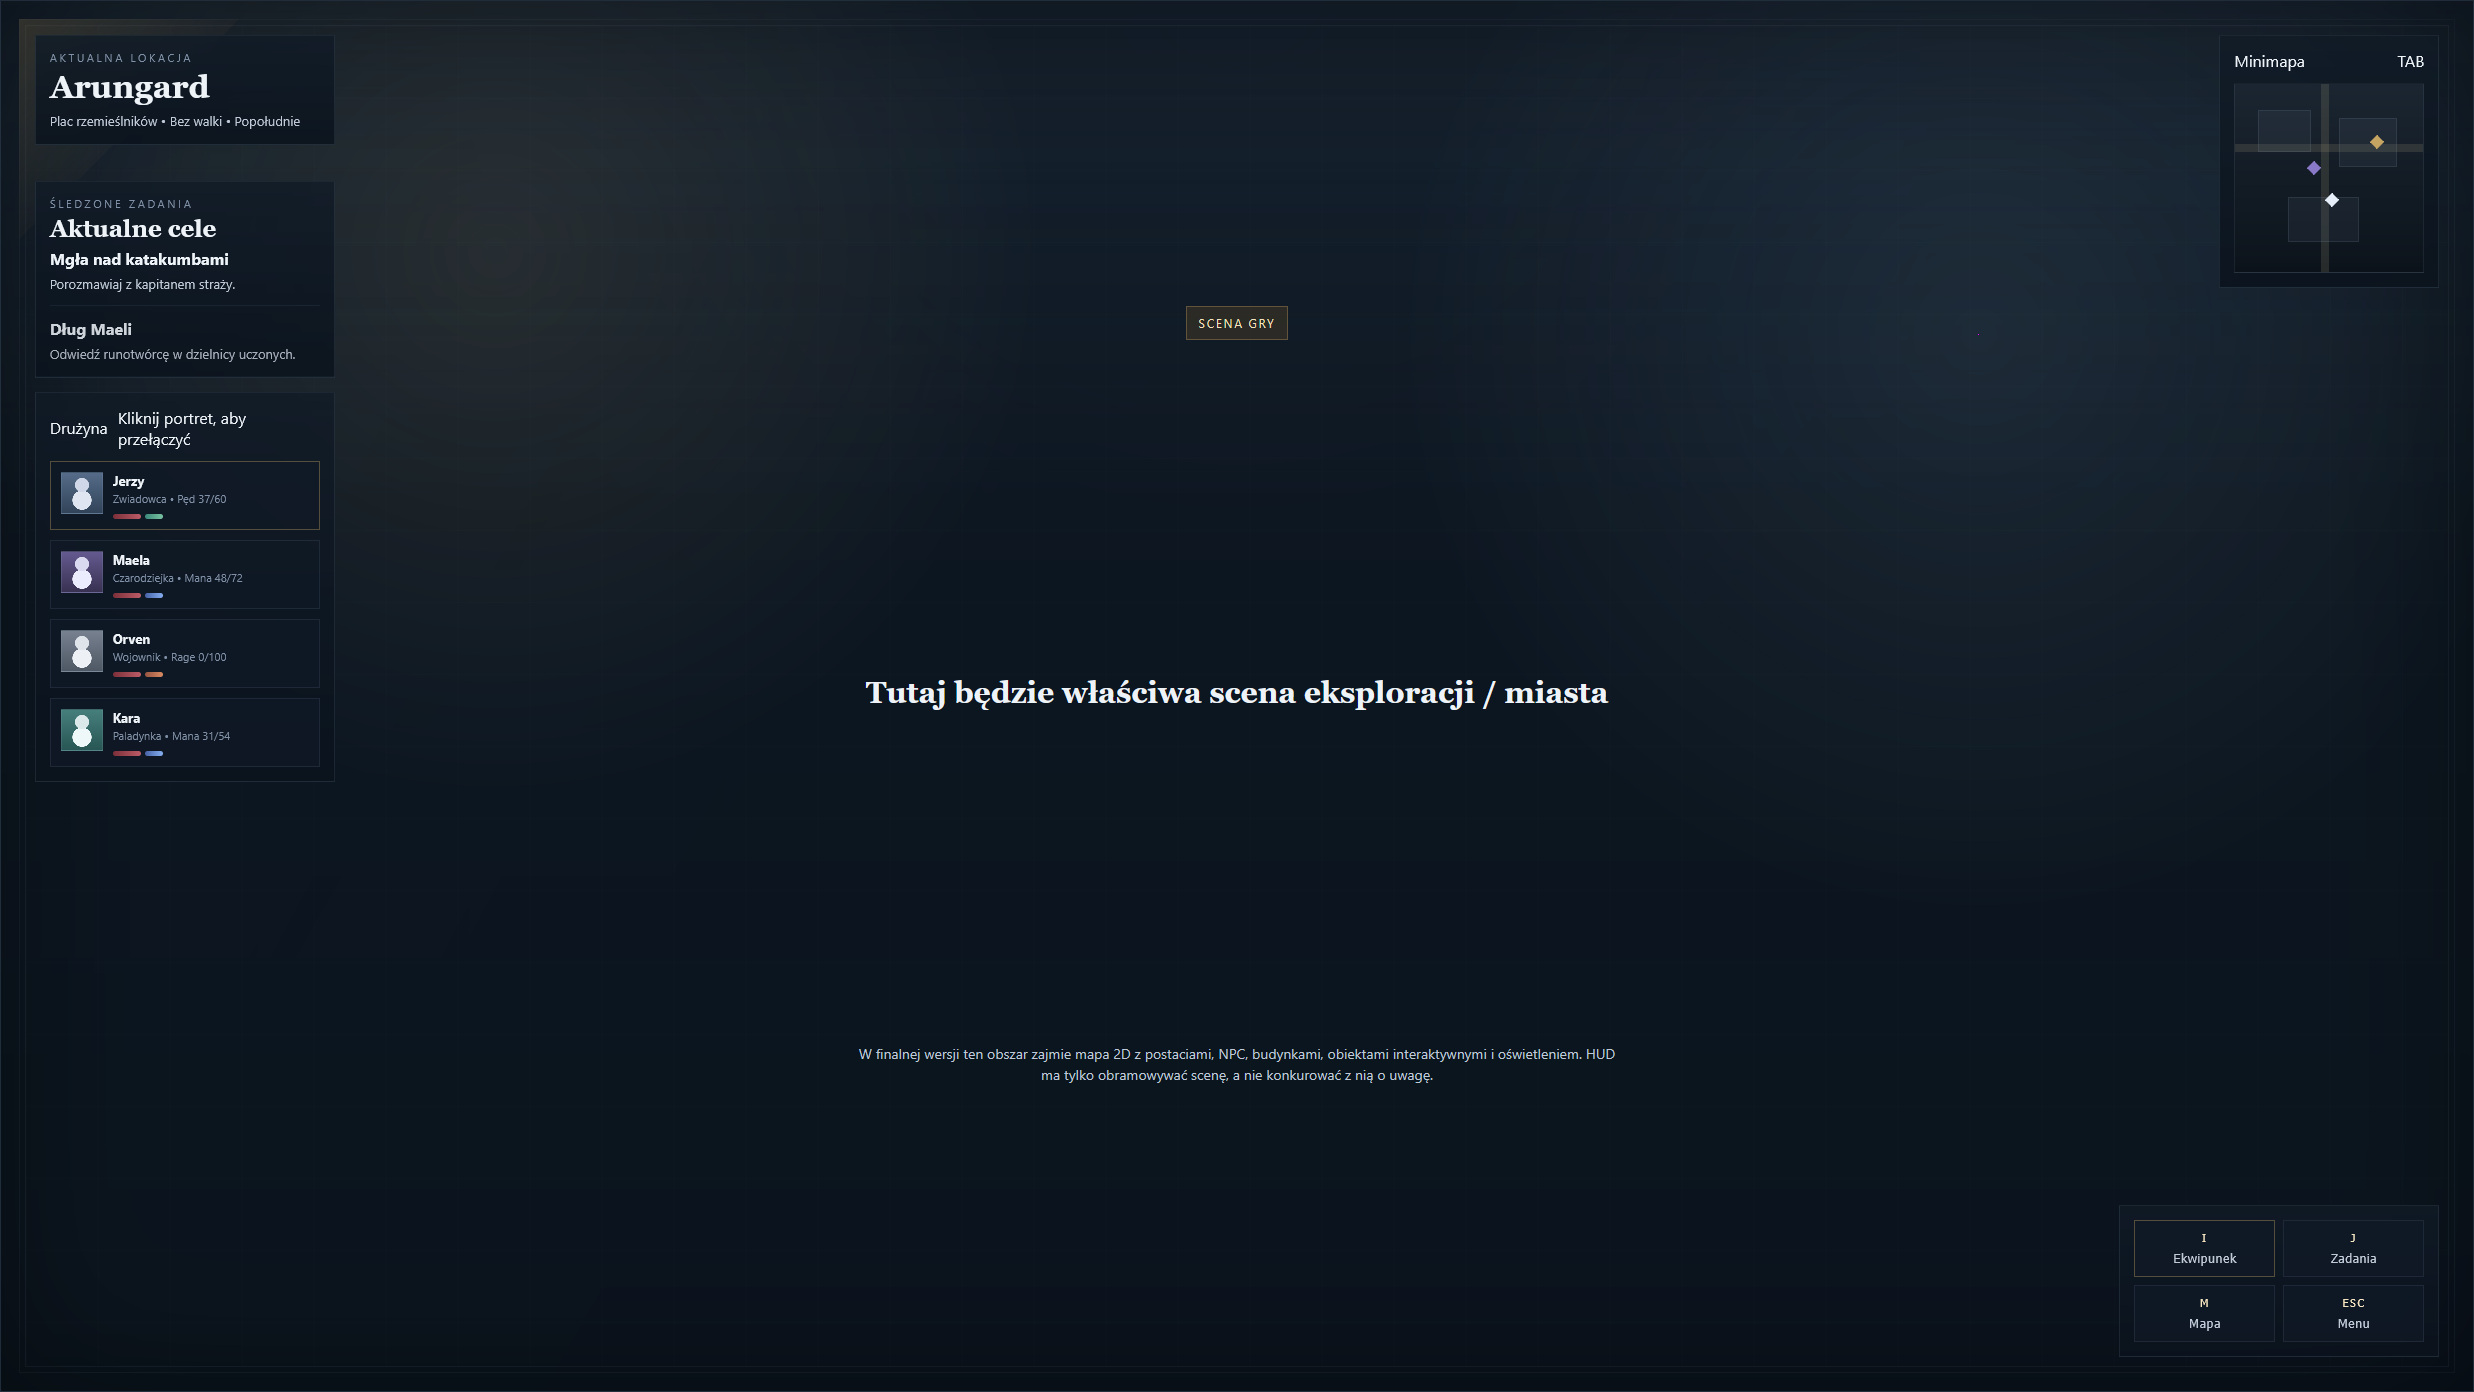
\includegraphics[width=\textwidth]{figures/gui/ui-exploration.png}
    \caption{Widok eksploracji i miasta}
    \wsizsource{Opracowanie własne}
\end{figure}

Widok eksploracji przedstawia podejście scene-first, w którym interfejs ograniczono do najważniejszych informacji: minimapy, aktywnych zadań, składu drużyny oraz podstawowych skrótów. Dzięki temu ekran nie zasłania przestrzeni gry i pozwala skupić uwagę użytkownika na otoczeniu.

\begin{figure}[H]
    \centering
    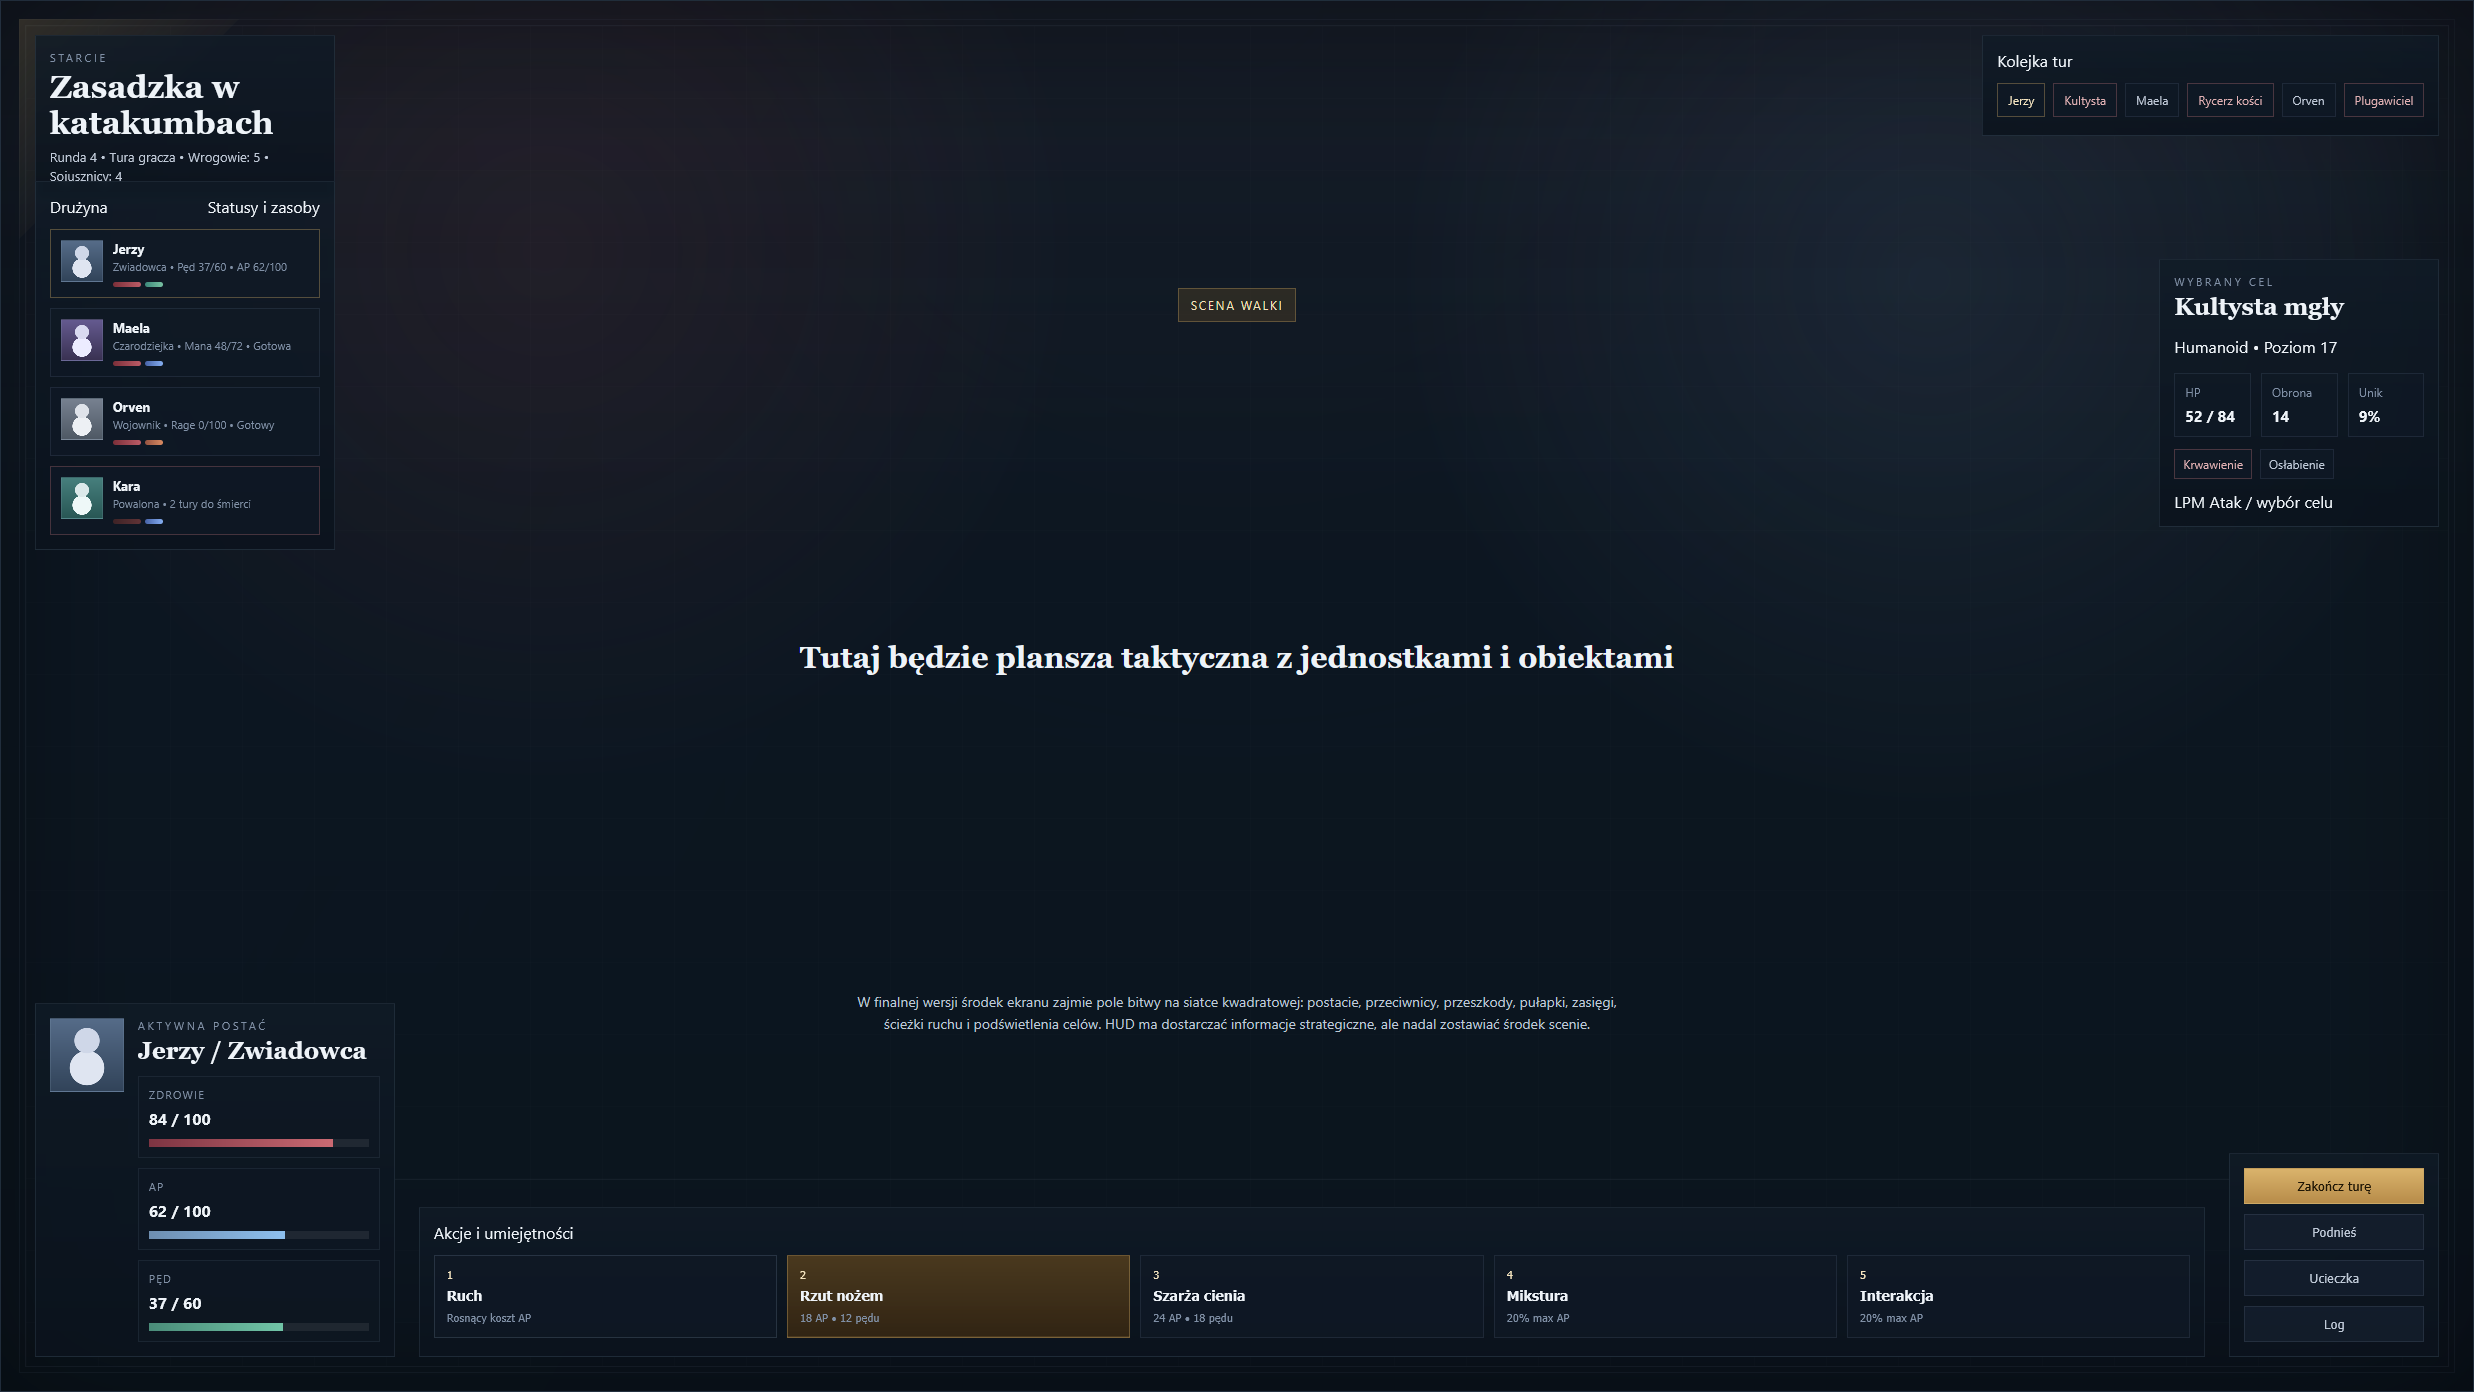
\includegraphics[width=\textwidth]{figures/gui/ui-combat-hud.png}
    \caption{Widok interfejsu walki}
    \wsizsource{Opracowanie własne}
\end{figure}

Interfejs walki zachowuje tę samą zasadę, jednak wzbogacono go o elementy strategiczne, takie jak kolejka tur, pasek umiejętności, panel aktywnej postaci oraz informacje o aktualnym celu. Rozmieszczenie tych elementów przy obrzeżach ekranu umożliwia jednoczesne śledzenie sytuacji taktycznej oraz samego pola bitwy.

\begin{figure}[H]
    \centering
    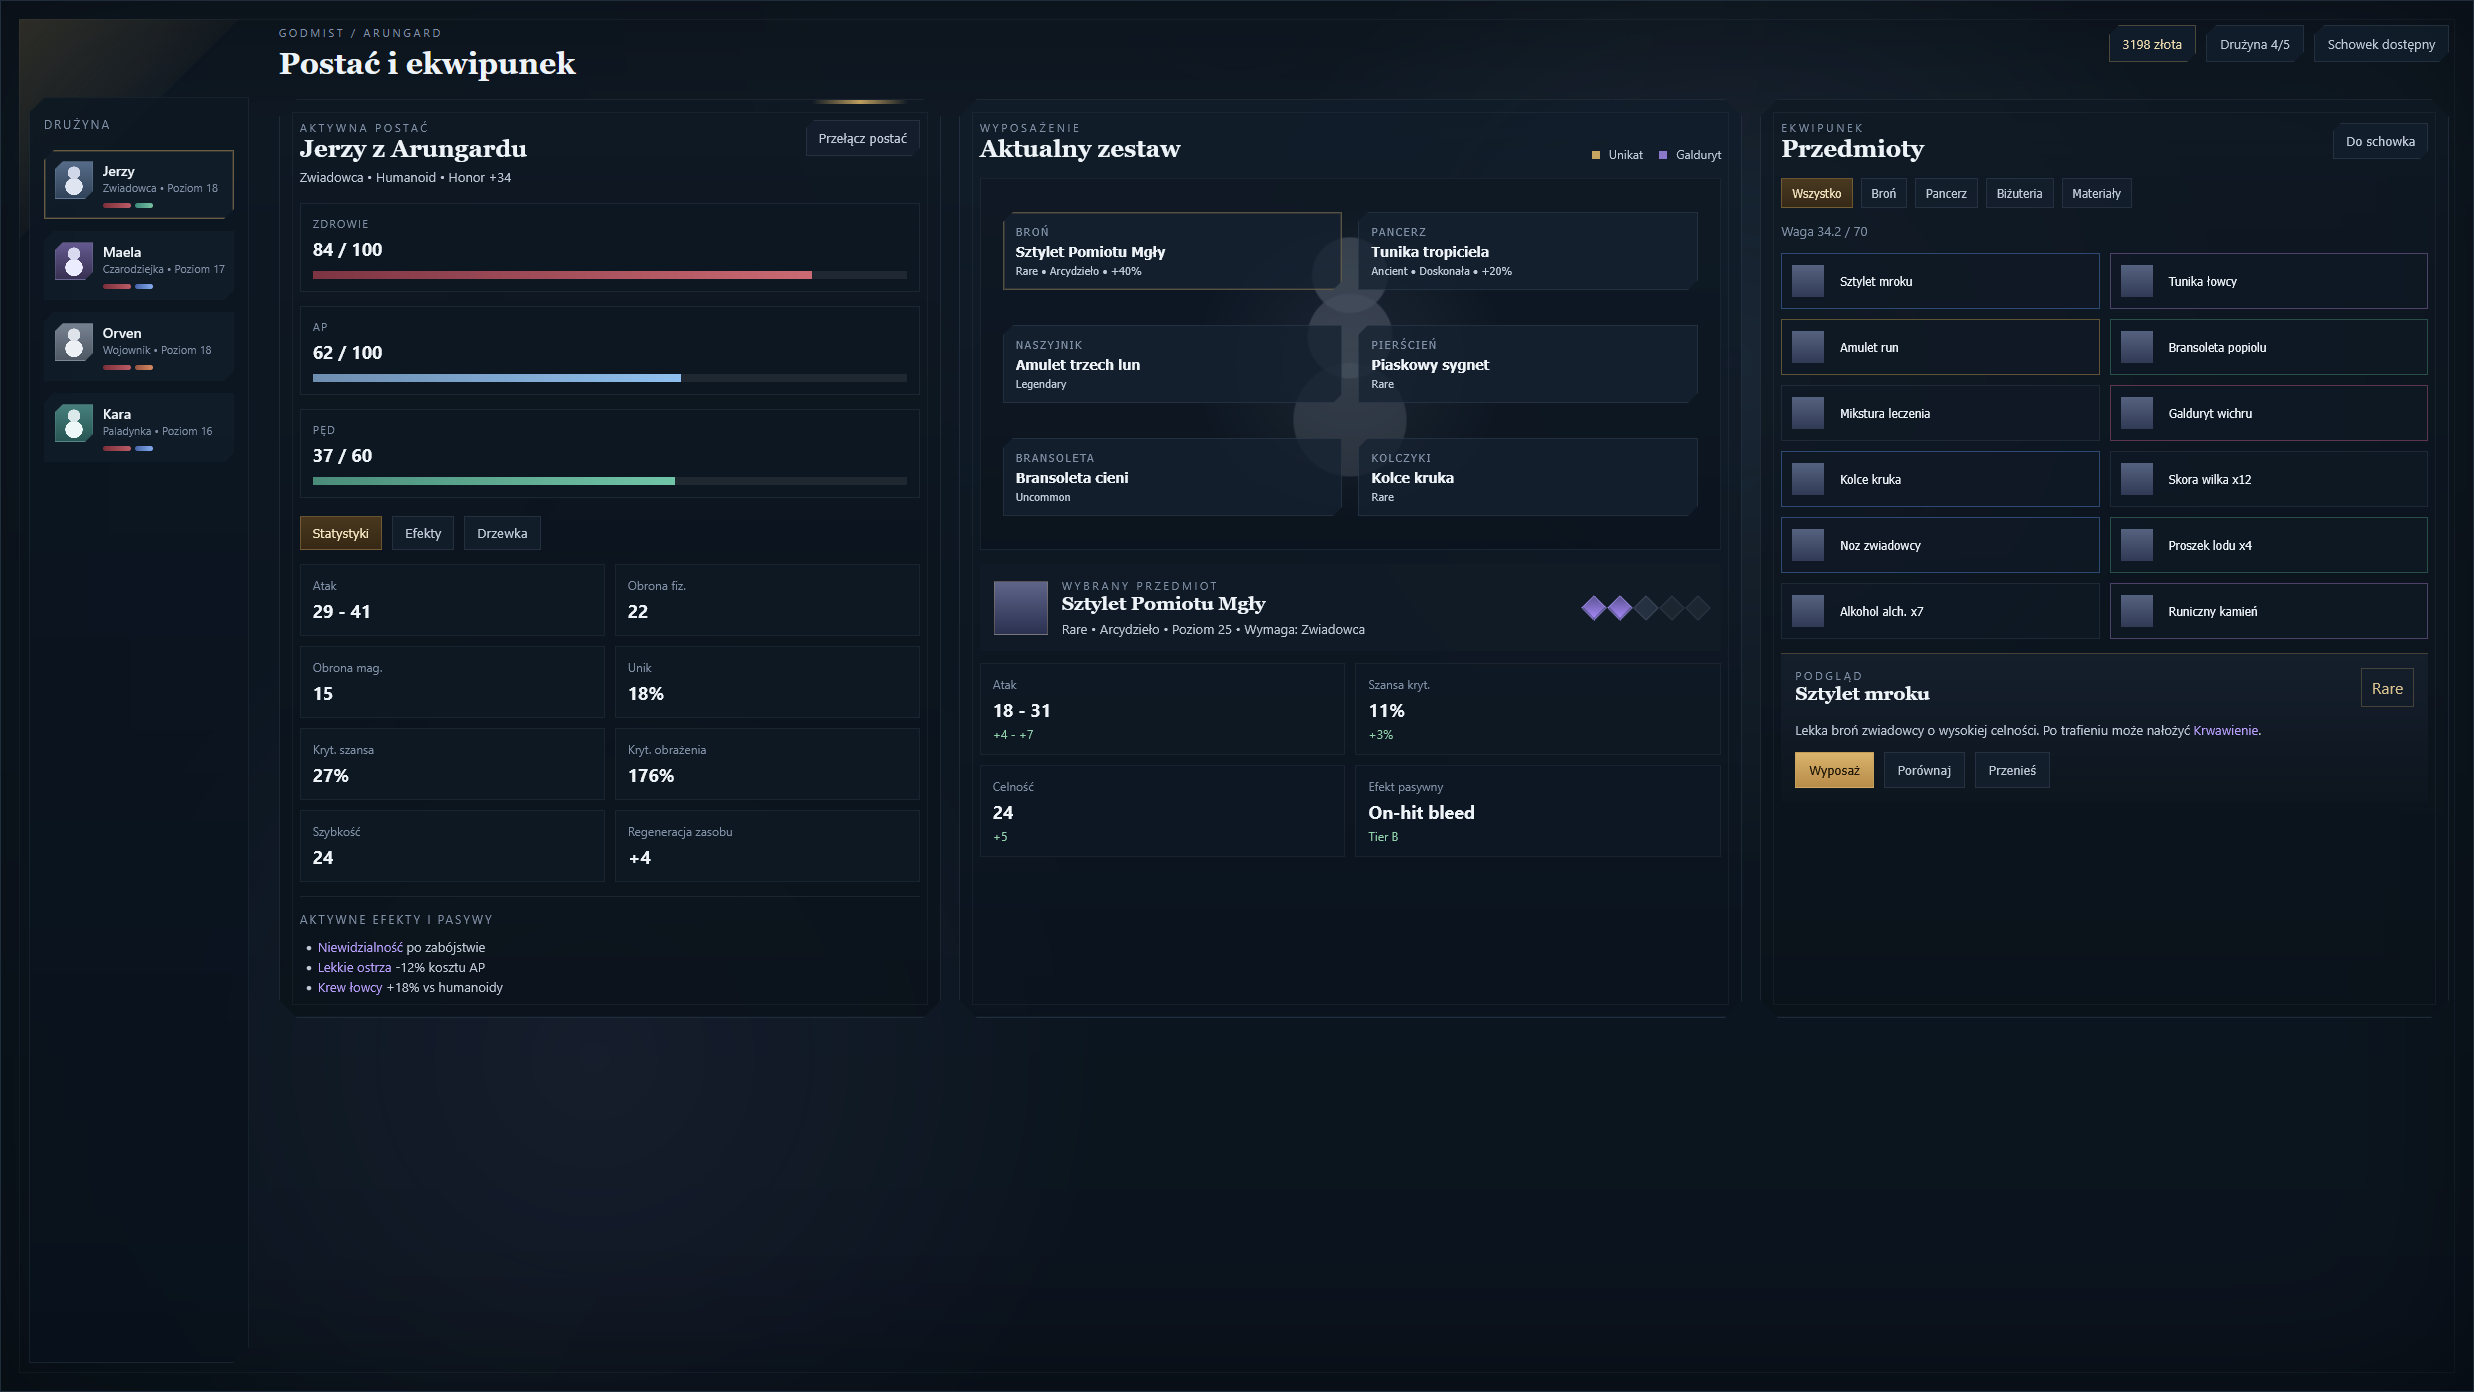
\includegraphics[width=\textwidth]{figures/gui/ui-character-equipment.png}
    \caption{Widok postaci i ekwipunku}
    \wsizsource{Opracowanie własne}
\end{figure}

Okno postaci i ekwipunku umożliwia przegląd statystyk, aktualnie założonych przedmiotów oraz zawartości ekwipunku. Centralnym elementem kompozycji jest sekcja wyposażenia postaci, natomiast informacje pomocnicze rozmieszczono po bokach w celu zachowania czytelności.

\begin{figure}[H]
    \centering
    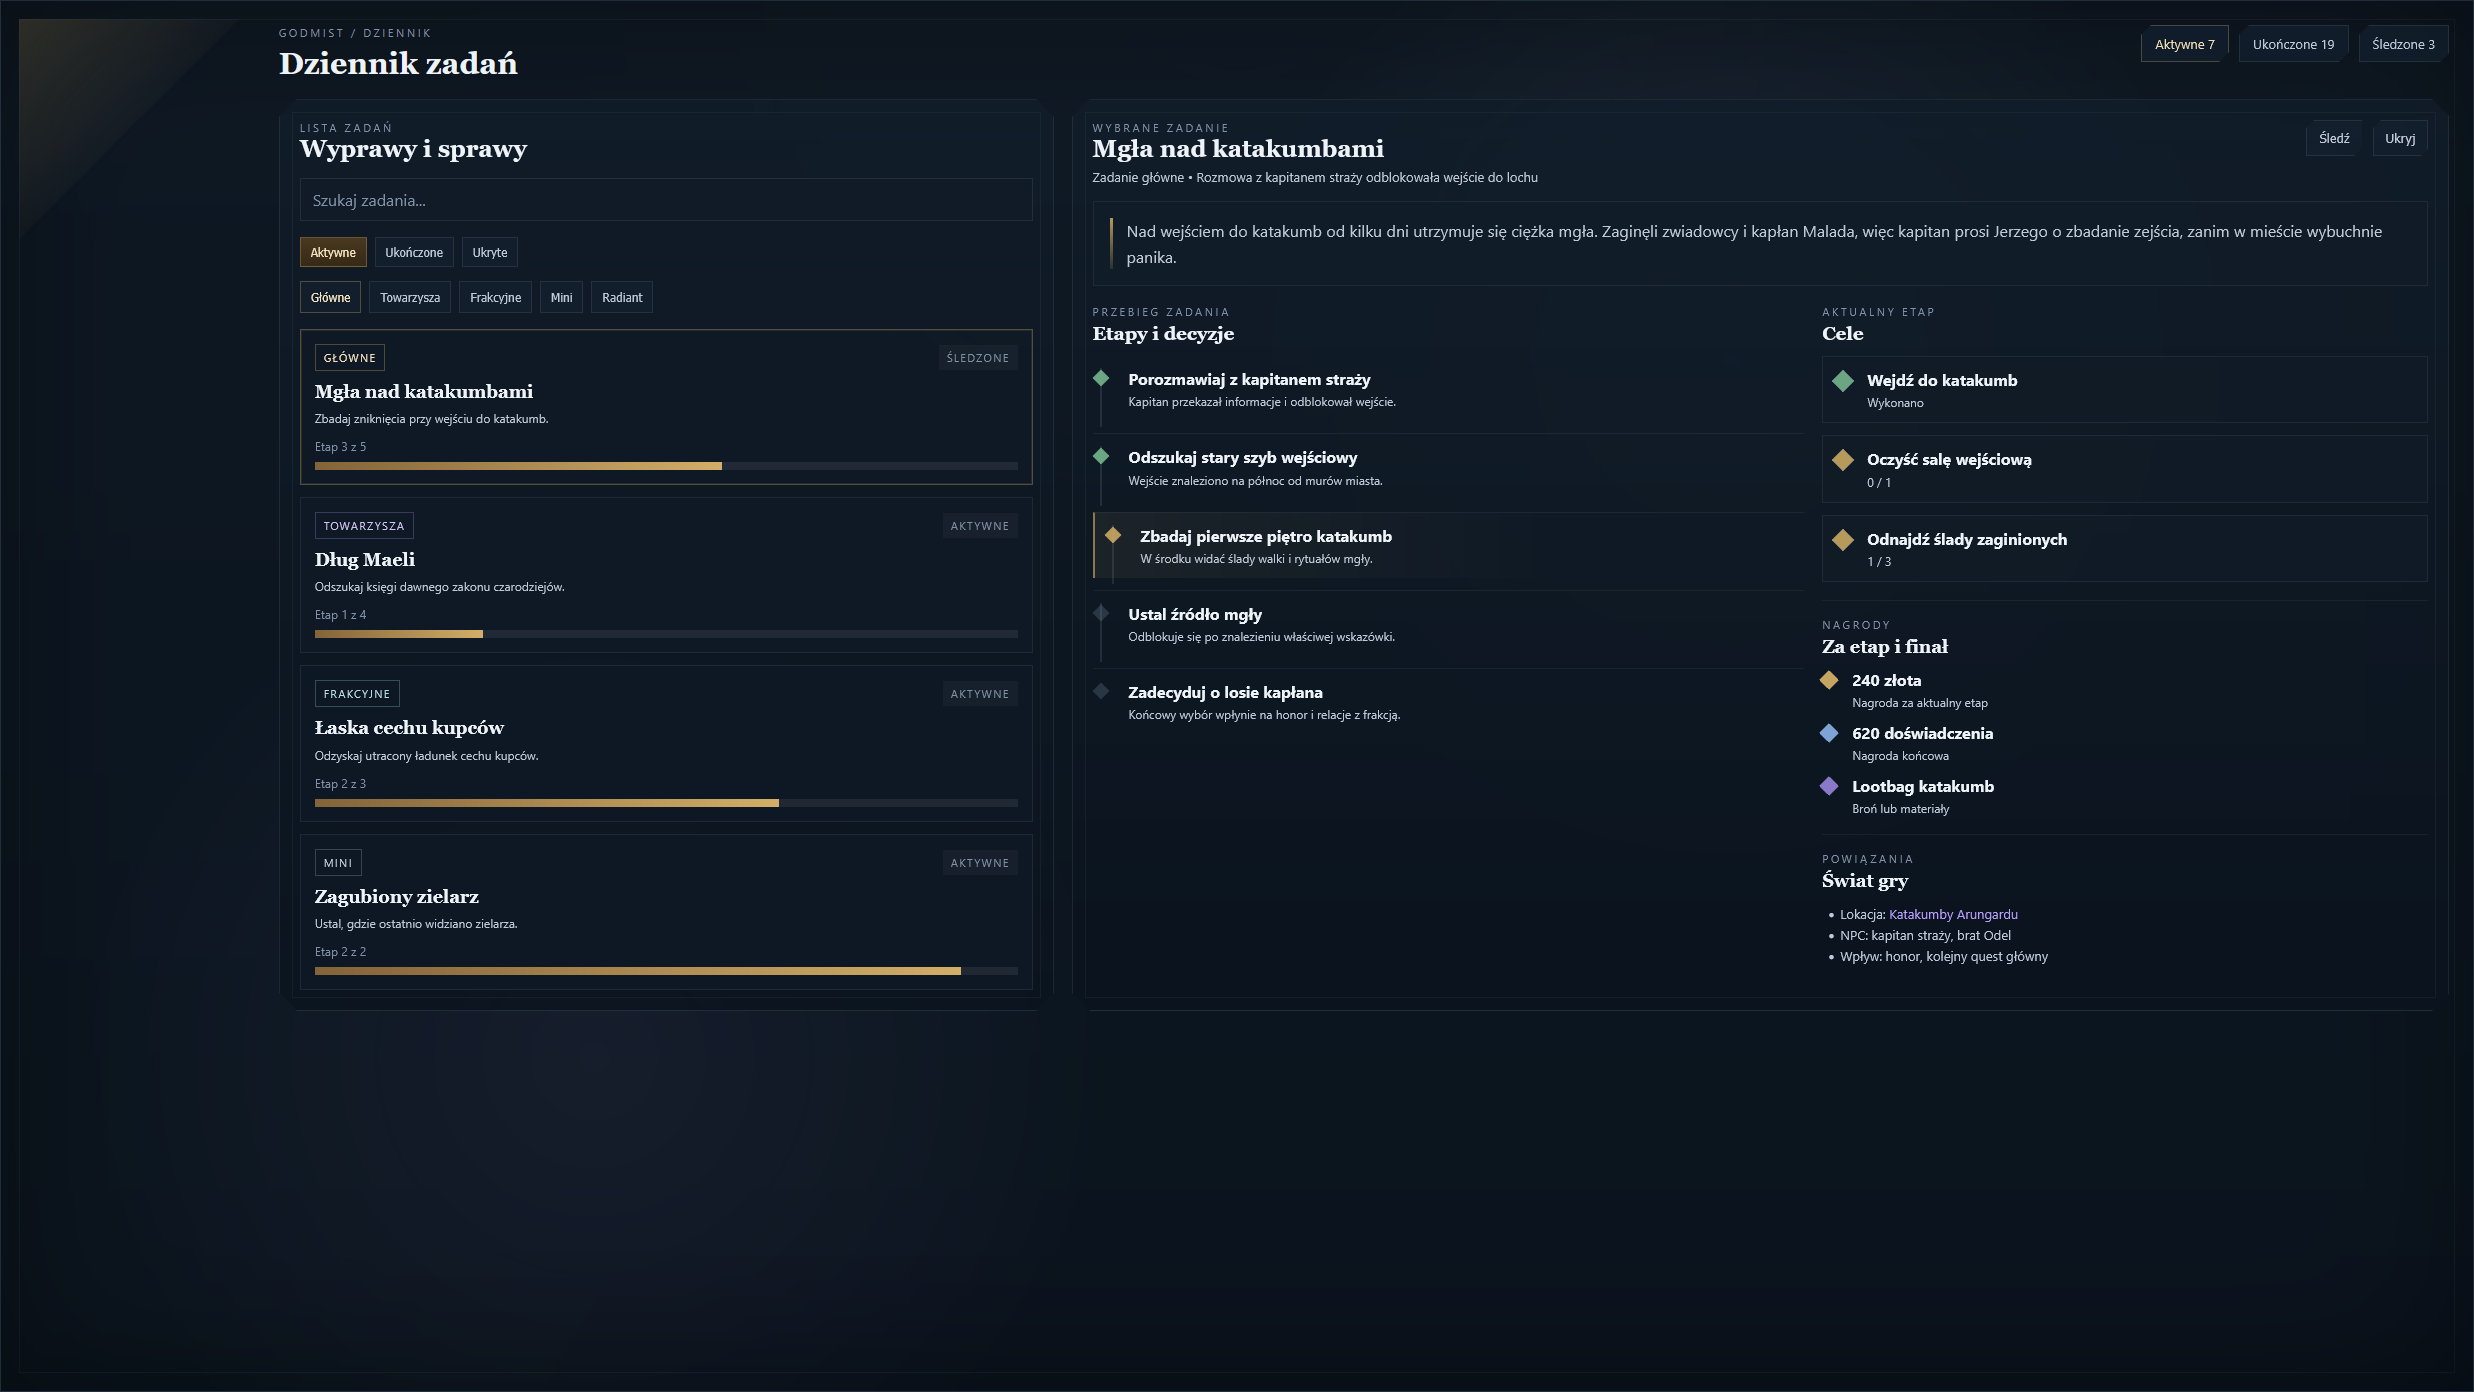
\includegraphics[width=\textwidth]{figures/gui/ui-quest-journal.png}
    \caption{Widok dziennika zadań}
    \wsizsource{Opracowanie własne}
\end{figure}

Dziennik zadań grupuje informacje o aktywnych i ukończonych misjach, ich etapach, nagrodach oraz powiązaniach ze światem gry. Układ kolumnowy pozwala oddzielić listę zadań od szczegółów aktualnie wybranego wpisu.

\begin{figure}[H]
    \centering
    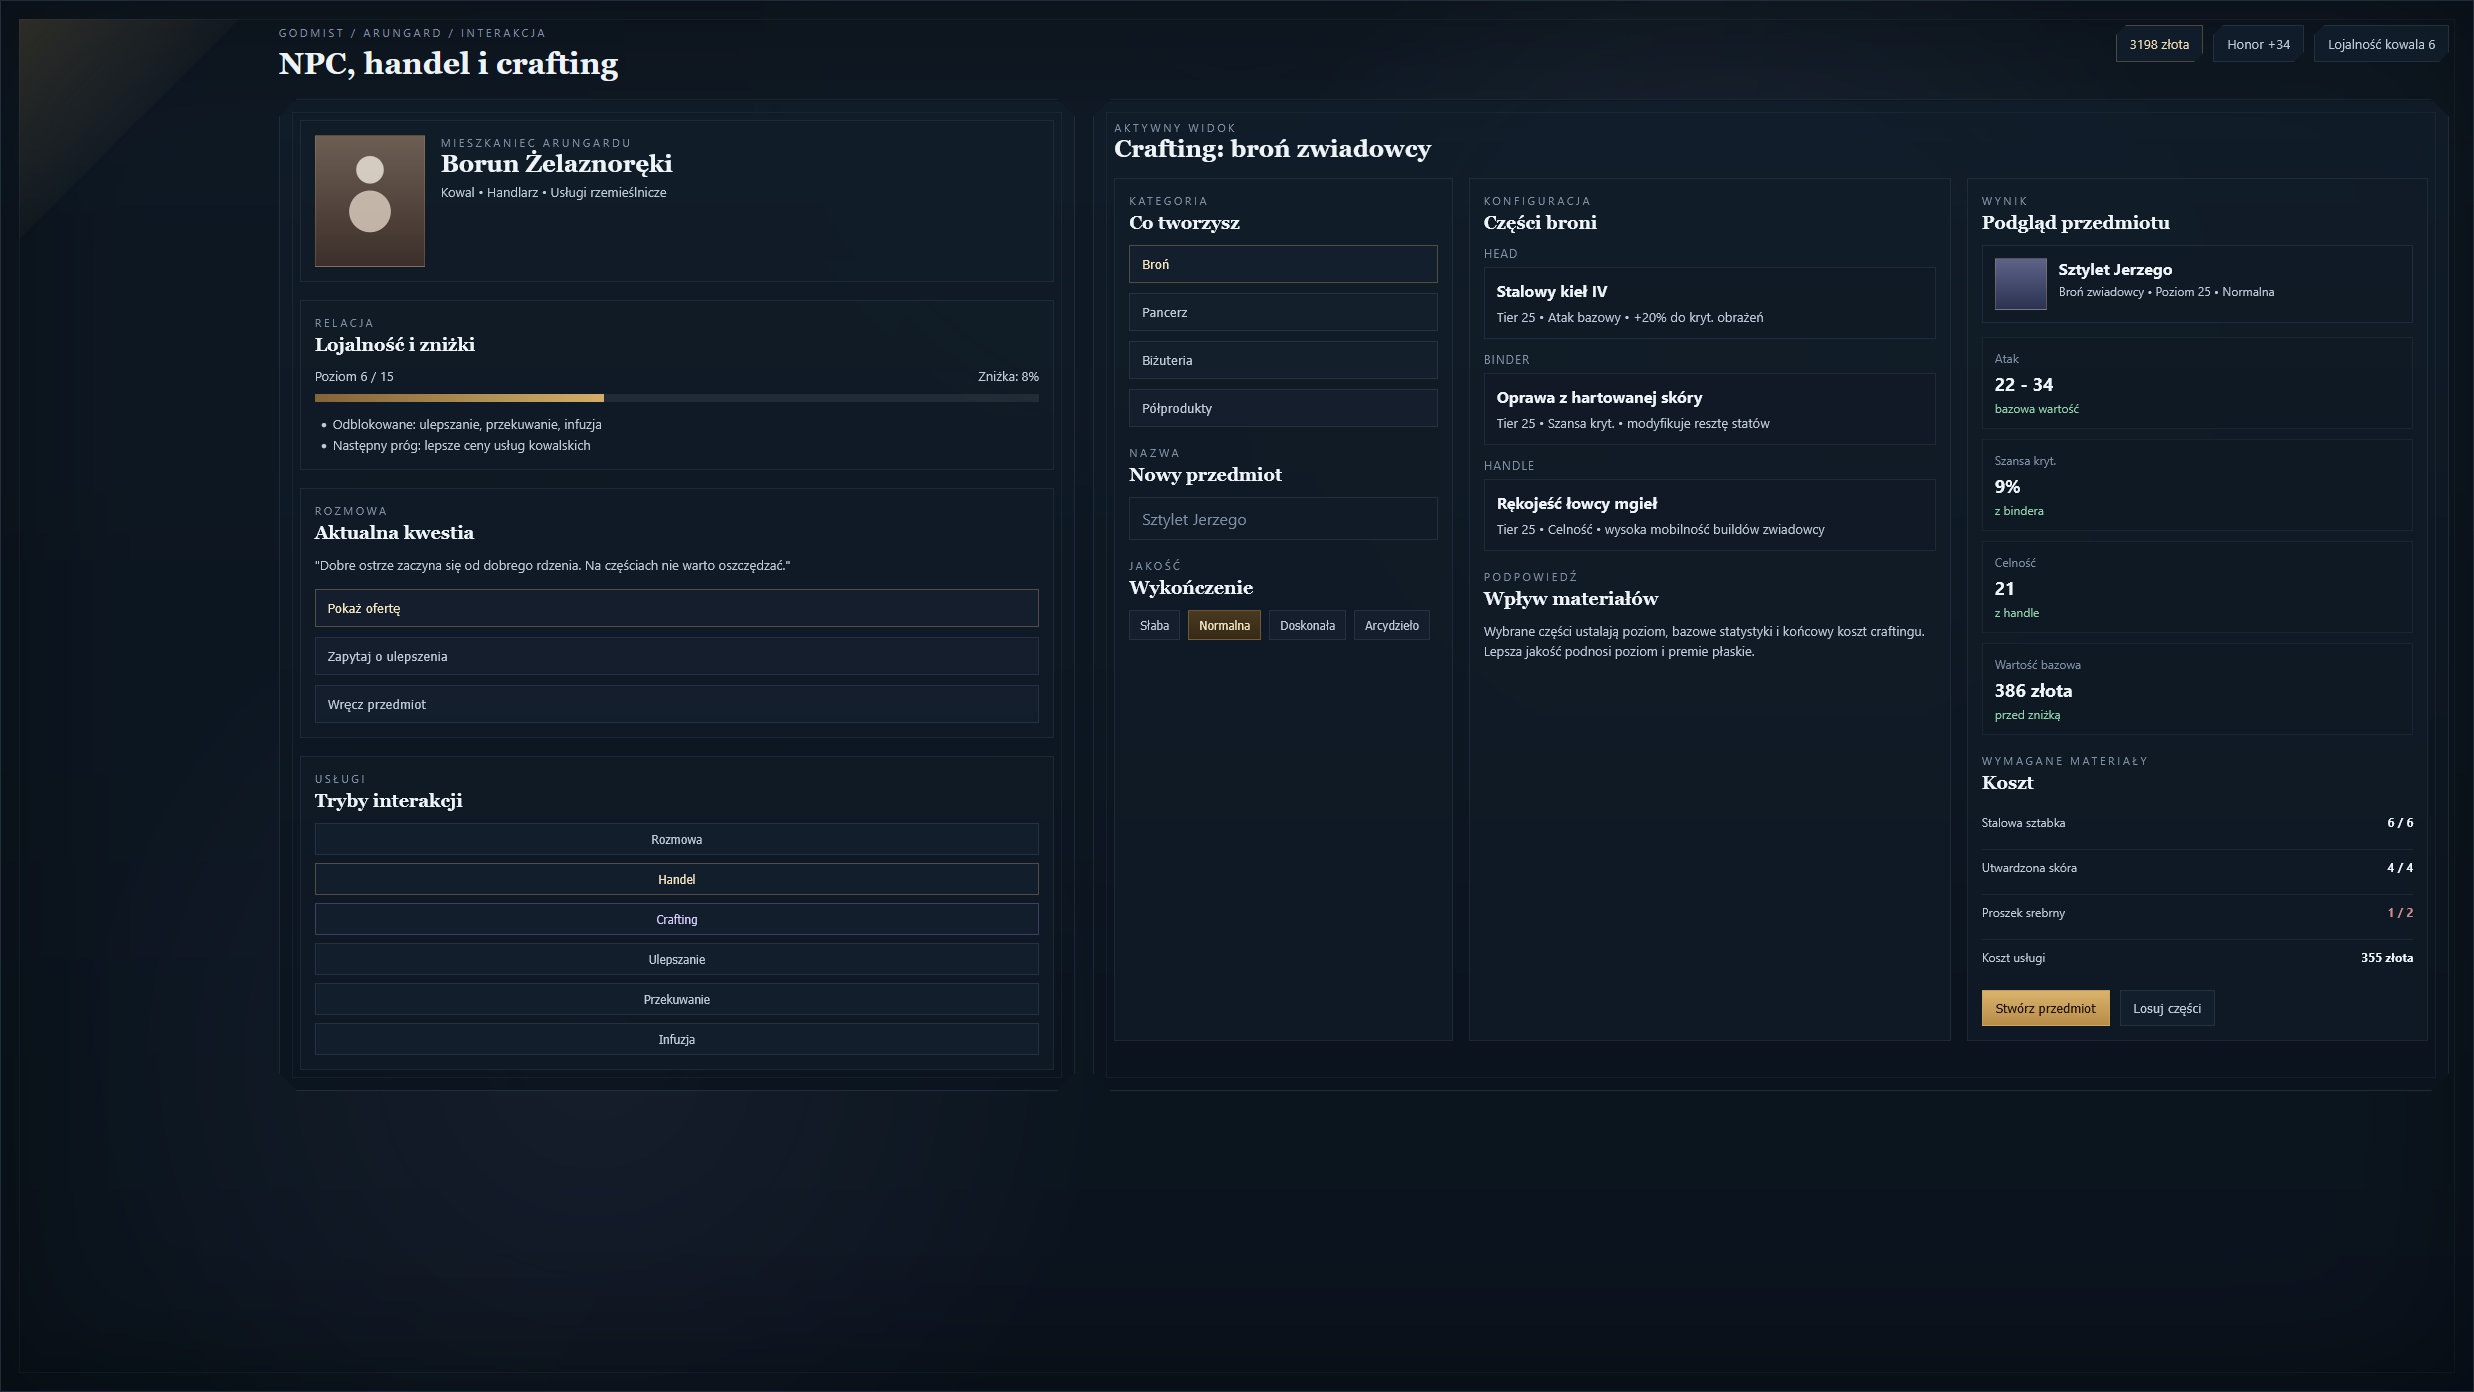
\includegraphics[width=\textwidth]{figures/gui/ui-npc-dialog.png}
    \caption{Widok interakcji z NPC}
    \wsizsource{Opracowanie własne}
\end{figure}

Okno interakcji z NPC stanowi wspólną bazę dla rozmowy, handlu oraz craftingu. Takie rozwiązanie upraszcza obsługę systemu i pozwala zachować spójność wizualną między różnymi usługami oferowanymi przez postacie niezależne.

\section{Propozycja testów}
\label{sec:propozycja-testow}

Ze względu na złożoność systemu \emph{Godmist} proces weryfikacji poprawności działania powinien obejmować kilka poziomów testowania. Oprócz sprawdzenia podstawowych funkcji dostępnych dla gracza konieczne jest również potwierdzenie poprawnej współpracy pomiędzy modułami systemu, prawidłowego działania zapisu i odczytu stanu gry oraz akceptowalnej wydajności rozwiązania. W niniejszej sekcji przedstawiono przykładowe scenariusze testowe, które mogą zostać wykorzystane podczas dalszej realizacji projektu.

Przedstawione przypadki testowe mają charakter projektowy. Oznacza to, że nie są jeszcze raportem z wykonanych testów, lecz propozycją zestawu sprawdzeń, które pozwolą zweryfikować zgodność implementacji z założeniami systemu. Dla czytelności testy podzielono na testy funkcjonalne, integracyjne, testy zapisu i odczytu oraz testy wydajnościowe i niezawodnościowe.

\subsection{Testy funkcjonalne}
\label{subsec:testy-funkcjonalne}

Testy funkcjonalne mają na celu sprawdzenie, czy system poprawnie realizuje najważniejsze funkcje widoczne z perspektywy użytkownika końcowego. Obejmują one między innymi rozpoczęcie gry, eksplorację lokacji, prowadzenie walki, rozwój postaci, korzystanie z ekwipunku oraz obsługę handlu i craftingu.

\begin{table}[H]
\centering
\caption{Przykładowe testy funkcjonalne systemu}
\label{tab:testy-funkcjonalne}
\begin{threeparttable}
\begin{tabularx}{\linewidth}{|p{1.6cm}|p{3.2cm}|X|X|X|}
\hline
\textbf{ID} & \textbf{Nazwa testu} & \textbf{Warunki początkowe} & \textbf{Kroki testowe} & \textbf{Oczekiwany rezultat} \\
\hline
TF-01 & Rozpoczęcie nowej gry & Aplikacja została uruchomiona, użytkownik znajduje się w menu głównym. & Wybrać opcję rozpoczęcia nowej gry. & System tworzy nową kampanię i przenosi gracza do początkowego stanu rozgrywki. \\
\hline
TF-02 & Eksploracja miasta & Gra została rozpoczęta, gracz znajduje się w mieście. & Poruszyć postać po mieście i wejść w interakcję z wybranym NPC. & Postać porusza się poprawnie, a interakcja z NPC otwiera odpowiedni panel lub dialog. \\
\hline
TF-03 & Rozpoczęcie walki w lochu & Gracz znajduje się w lochu i zbliża się do grupy przeciwników. & Wejść w zasięg przeciwnika inicjujący walkę. & System przełącza stan gry do trybu walki i inicjuje sesję combatową. \\
\hline
TF-04 & Użycie umiejętności w walce & Trwa walka, aktywna postać posiada wystarczające zasoby i punkty akcji. & Wybrać umiejętność i wskazać poprawny cel. & Umiejętność zostaje wykonana, a stan zasobów, punktów akcji i celu zostaje odpowiednio zaktualizowany. \\
\hline
TF-05 & Handel z NPC & Gracz znajduje się w mieście i posiada przedmiot oraz odpowiednią ilość złota. & Otworzyć sklep NPC, kupić oraz sprzedać wybrany przedmiot. & System poprawnie aktualizuje złoto, inventory gracza oraz stan sklepu i listy buyback. \\
\hline
TF-06 & Crafting przedmiotu & Gracz znajduje się przy odpowiednim NPC i posiada wymagane składniki. & Wybrać recepturę lub konfigurację przedmiotu i potwierdzić crafting. & System tworzy nowy przedmiot zgodnie z wybranymi parametrami i zużywa odpowiednie składniki. \\
\hline
TF-07 & Rozwój postaci & Postać posiada dostępne punkty rozwoju. & Otworzyć drzewko umiejętności i zainwestować punkt w wybrany node. & System zwiększa inwestycję w node, aktualizuje liczbę punktów i odblokowuje odpowiednie efekty. \\
\hline
\end{tabularx}
\wsizsource{Opracowanie własne}
\end{threeparttable}
\end{table}

\subsection{Testy integracyjne}
\label{subsec:testy-integracyjne}

Testy integracyjne służą do sprawdzenia poprawnej współpracy pomiędzy różnymi modułami systemu. W przypadku gry \emph{Godmist} ma to szczególne znaczenie, ponieważ wiele mechanik korzysta z tych samych danych runtime i oddziałuje na stan świata, postaci oraz przedmiotów.

\begin{table}[H]
\centering
\caption{Przykładowe testy integracyjne systemu}
\label{tab:testy-integracyjne}
\begin{threeparttable}
\begin{tabularx}{\linewidth}{|p{1.6cm}|p{3.2cm}|X|X|X|}
\hline
\textbf{ID} & \textbf{Nazwa testu} & \textbf{Warunki początkowe} & \textbf{Kroki testowe} & \textbf{Oczekiwany rezultat} \\
\hline
TI-01 & Walka i efekty statusu & Trwa walka, aktywna postać posiada umiejętność nakładającą status. & Użyć umiejętności nakładającej efekt statusu na przeciwnika. & System poprawnie nakłada status, zapisuje go w stanie postaci i uwzględnia jego działanie w kolejnych turach. \\
\hline
TI-02 & Ekwipunek i statystyki postaci & Postać posiada przedmiot zwiększający statystyki. & Założyć przedmiot na postać, a następnie go zdjąć. & Statystyki postaci zmieniają się po założeniu przedmiotu i wracają do poprzednich wartości po jego zdjęciu. \\
\hline
TI-03 & Quest i stan świata & Aktywna jest misja wymagająca interakcji z obiektem lub NPC. & Wykonać czynność wymaganą przez quest. & System aktualizuje postęp questa oraz odpowiednie flagi świata lub questa. \\
\hline
TI-04 & Loch i system walki & Gracz eksploruje loch zawierający encounter. & Wejść do pomieszczenia z przeciwnikami i ukończyć walkę. & System aktualizuje stan encountera w lochu i oznacza go jako ukończony. \\
\hline
TI-05 & Crafting i inventory & Gracz posiada wymagane materiały do craftingu. & Wytworzyć przedmiot u odpowiedniego NPC. & Materiały zostają zużyte, a nowy przedmiot trafia do odpowiedniego inventory. \\
\hline
\end{tabularx}
\wsizsource{Opracowanie własne}
\end{threeparttable}
\end{table}

\subsection{Testy zapisu i odczytu}
\label{subsec:testy-zapisu-i-odczytu}

Ze względu na przyjęty model trwałości danych oparty na plikach JSON, testy zapisu i odczytu należą do najważniejszych w całym projekcie. Ich celem jest weryfikacja, czy stan gry po zapisaniu i ponownym wczytaniu pozostaje zgodny ze stanem sprzed zakończenia sesji.

\begin{table}[H]
\centering
\caption{Przykładowe testy zapisu i odczytu}
\label{tab:testy-zapis-odczyt}
\begin{threeparttable}
\begin{tabularx}{\linewidth}{|p{1.6cm}|p{3.2cm}|X|X|X|}
\hline
\textbf{ID} & \textbf{Nazwa testu} & \textbf{Warunki początkowe} & \textbf{Kroki testowe} & \textbf{Oczekiwany rezultat} \\
\hline
TZ-01 & Zapis i wczytanie postaci & Postać posiada określony poziom, statystyki, ekwipunek i aktywne efekty. & Zapisać grę, zamknąć aplikację, a następnie wczytać zapis. & Po wczytaniu system odtwarza stan postaci zgodny ze stanem sprzed zapisu. \\
\hline
TZ-02 & Zapis i wczytanie lochu & Gracz znajduje się w lochu, odwiedził część pomieszczeń i ukończył wybrane encountery. & Zapisać grę i następnie wczytać zapis. & Stan lochu, w tym odwiedzone pomieszczenia i ukończone spotkania, zostaje odtworzony poprawnie. \\
\hline
TZ-03 & Zapis i wczytanie questów & Gracz posiada aktywne questy z częściowym postępem. & Zapisać grę i ponownie ją wczytać. & System poprawnie odtwarza status questów, cele oraz postęp wykonania. \\
\hline
TZ-04 & Zapis stanu NPC i handlu & NPC posiada określony poziom lojalności oraz stan sklepu i buybacku. & Zapisać grę po dokonaniu transakcji, a następnie ją wczytać. & Lojalność NPC, oferta sklepu i buyback pozostają zgodne z zapisanym stanem. \\
\hline
TZ-05 & Zapis schowka & W schowku znajdują się różne przedmioty. & Odłożyć przedmioty do schowka, zapisać grę i ponownie ją wczytać. & Schowek po wczytaniu zawiera ten sam zestaw przedmiotów. \\
\hline
\end{tabularx}
\wsizsource{Opracowanie własne}
\end{threeparttable}
\end{table}

\subsection{Testy wydajnościowe i niezawodnościowe}
\label{subsec:testy-wydajnosciowe}

Testy wydajnościowe i niezawodnościowe mają na celu ocenę stabilności systemu oraz sprawdzenie, czy podstawowe operacje nie powodują zauważalnych opóźnień lub błędów przy większej złożoności stanu gry. W przypadku projektu \emph{Godmist} istotne jest zwłaszcza zachowanie systemu przy rozbudowanym ekwipunku, wielu aktywnych efektach oraz przy obsłudze proceduralnie generowanych lochów.

\begin{table}[H]
\centering
\caption{Przykładowe testy wydajnościowe i niezawodnościowe}
\label{tab:testy-wydajnosciowe}
\begin{threeparttable}
\begin{tabularx}{\linewidth}{|p{1.6cm}|p{3.2cm}|X|X|X|}
\hline
\textbf{ID} & \textbf{Nazwa testu} & \textbf{Warunki początkowe} & \textbf{Kroki testowe} & \textbf{Oczekiwany rezultat} \\
\hline
TW-01 & Ładowanie lochu proceduralnego & System jest gotowy do wejścia do lochu. & Wygenerować i załadować loch proceduralny. & Loch zostaje wygenerowany i załadowany bez błędów, a czas oczekiwania pozostaje akceptowalny dla użytkownika. \\
\hline
TW-02 & Zapis dużego stanu gry & Gra zawiera rozwiniętą drużynę, dużą liczbę przedmiotów i aktywnych questów. & Wykonać zapis gry. & System zapisuje stan bez błędów i bez zauważalnego zawieszenia aplikacji. \\
\hline
TW-03 & Wczytanie dużego stanu gry & Istnieje zapis obejmujący rozbudowany stan świata i postaci. & Wczytać zapis gry. & System poprawnie odtwarza stan gry bez utraty danych i bez krytycznych opóźnień. \\
\hline
TW-04 & Stabilność długiej sesji gry & Użytkownik wykonuje wiele walk, interakcji i zapisów podczas jednej sesji. & Przeprowadzić dłuższą rozgrywkę obejmującą wiele przejść między modułami. & System zachowuje stabilność i nie wykazuje krytycznych błędów ani utraty spójności danych. \\
\hline
\end{tabularx}
\wsizsource{Opracowanie własne}
\end{threeparttable}
\end{table}

Przedstawiony zestaw testów nie wyczerpuje wszystkich możliwych scenariuszy weryfikacji systemu, ale stanowi reprezentatywną podstawę do dalszego planowania procesu testowania. Uwzględnia on zarówno działania wykonywane bezpośrednio przez użytkownika, jak i poprawność współpracy modułów, trwałość danych oraz stabilność techniczną systemu.

\section{Podsumowanie rozdziału}
\label{sec:podsumowanie-rozdzialu-3}

W niniejszym rozdziale przedstawiono założenia dotyczące interfejsu użytkownika projektowanego systemu oraz zaproponowano przykładowe scenariusze testowe, które mogą zostać wykorzystane podczas dalszej realizacji projektu. Omówiono najważniejsze widoki GUI związane z menu głównym, miastem, eksploracją lochu, walką oraz zarządzaniem ekwipunkiem i rozwojem postaci. Pozwoliło to określić, w jaki sposób użytkownik będzie komunikował się z systemem w różnych kontekstach rozgrywki.

Dodatkowo zaprezentowano propozycję testów funkcjonalnych, integracyjnych, testów zapisu i odczytu oraz testów wydajnościowych i niezawodnościowych. Dzięki temu projekt został uzupełniony o perspektywę weryfikacji poprawności działania poszczególnych modułów. Przedstawione elementy stanowią praktyczne dopełnienie wcześniejszych rozdziałów poświęconych analizie, wymaganiom oraz modelowi systemu.